\begin{figure}[H]
\centering
\begin{subfigure}[t]{0.48\textwidth}
\centering    
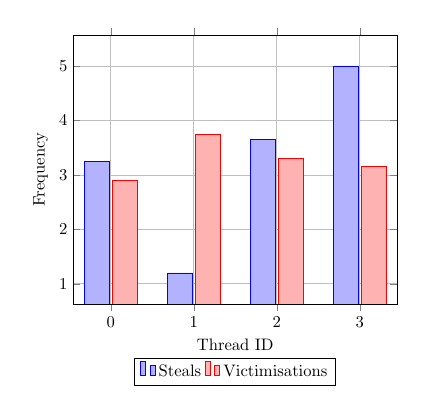
\begin{tikzpicture}[scale=0.6,baseline]
\begin{axis}[
    grid=major,
    x tick label style={
    /pgf/number format/1000 sep=},
    ylabel=Frequency,
    xlabel=Thread ID,
    enlargelimits=0.15,
    legend style={at={(0.5,-0.2)},
    anchor=north,legend columns=-1},
    ybar,
    bar width=15pt,
]
\addplot
    coordinates {
        (0,3.25)
        (1,1.2)
        (2,3.65)
        (3,5) 
    };
\addplot
    coordinates {
        (0,2.9)
        (1,3.75)
        (2,3.3)
        (3,3.15)
    };
\legend{Steals,Victimisations}
\end{axis}
\end{tikzpicture}
\caption{Steal count and victimisation count per thread.}
\label{fig:barstvvi}
\end{subfigure}
~ %spacer
\begin{subfigure}[t]{0.48\textwidth}
  \centering
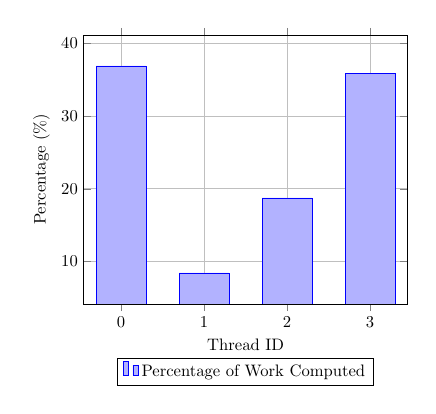
\begin{tikzpicture}[scale=0.6,baseline]
\begin{axis}[
    grid=major,
    x tick label style={
    /pgf/number format/1000 sep=},
    ylabel=Percentage (\%),
    xlabel=Thread ID,
    enlargelimits=0.15,
    legend style={at={(0.5,-0.2)},
    anchor=north,legend columns=-1},
    ybar,
    bar width=30pt,
]
\addplot
    coordinates {
        (0,36.9025)
        (1,8.431)
        (2,18.7375)
        (3,35.929) 
    };
\legend{Percentage of Work Computed}
\end{axis}
\end{tikzpicture}
\caption{Percentage of total work-load computed per thread.}
\label{fig:barworkperthread}
\end{subfigure}
% full caption
\caption{
    Sub-figure \ref{fig:barstvvi} shows a bar chart to display the average frequency of steal operations and the average 
    frequency of victimisations, per thread id, over twenty test runs.
    Sub-figure \ref{fig:barworkperthread} shows a bar chart to show the average percentage of the raster-plane computed
    by each thread over the same twenty test runs.
}
\label{fig:stealvictbar}
\end{figure}
